%GLOSSARYB
%%%%%%%%%%%%%%%%%%%%%%%%%%%
%%%% Put the following at the top of each .tex file  %
\pagestyle{fancy}
\setcounter{page}{1}
\rhead{Glossary Part B}
\lhead{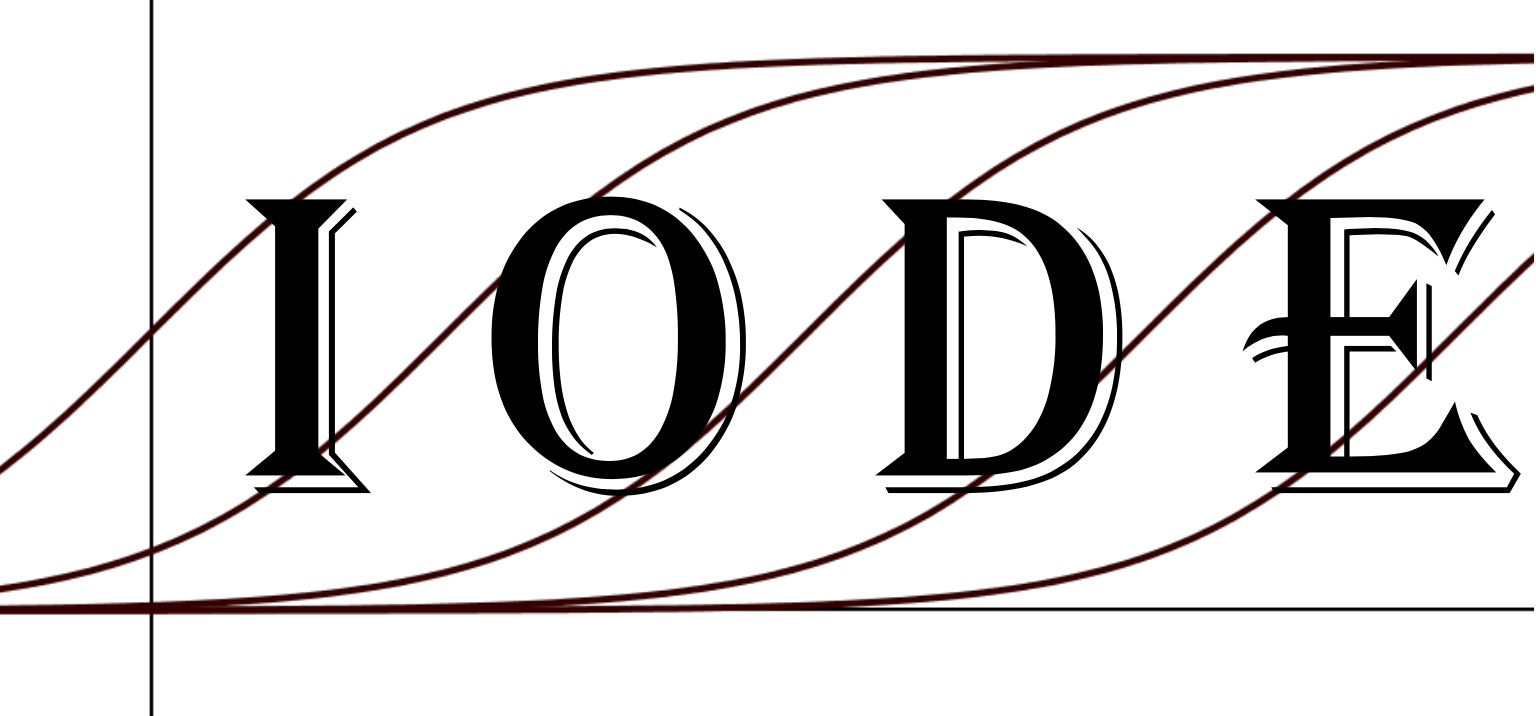
\includegraphics[width=1.25cm]{IODE-logo.png}}
\rfoot{Glossary Part B Page \thepage}
\lfoot{}
\cfoot{}
\fancypagestyle{firstfooter}{\footskip = 50pt}
\renewcommand{\footrulewidth}{.4pt}
%%%%%%%%%%%%%%%%%%%%%%%%%%%
\vspace*{-20pt} \thispagestyle{firstfooter}
\pagebegin{Glossary for Systems, Second Order, and Nonlinear DEs}
\begin{description}
\item[Characteristic equation:] A polynomial equation corresponding to a second order linear differential equation that is used to help find solutions.  
\item[Damping, Overdamped, Undamped:] Damping is the presence of a friction-like force in the system. Undamped is the lack of friction-like in the system. A system is called overdamped if the friction-like parameter exceeds a certain value determined by other parameters in the system.  
\item[Dependent (pertaining to linear algebraic equations):] A homogeneous system of two equations is dependent when it has infinitely many solutions.
\item[Differential equation:] A differential equation is also known as a \textbf{rate of change equation}. An equation for an unknown function in terms of its derivative. Suppose $y = y(t)$ is some unknown function, then a differential equation, or rate of change equation, would express the rate of change, $\frac{dy}{dt}$, in terms of $y$ and/or $t$. \textbf{First order} differential equation contains only the first derivative. \textbf{Second order} differential equations contains derivatives up to the second derivative. An \textbf{ordinary differential equation (ODE)} is a differential equation whose derivatives pertain to only one variable, typically derivatives with respect to time. A \textbf{partial differential equation (PDE)} is a differential equation whose derivatives pertain to multiple variables.
\item[Eigensolution:] A straight line solution formed from an eigenvalue, eigenvector pair.
\item[Eigenvalue:] The value of the exponent associated with any straight line solution to a system of differential equations.
\item[Homogeneous differential equation:] The following second order differential equation, $P(t)\frac{d^2y}{dt^2}+Q(t)\frac{dy}{dt}+R(t)y=G(t)$, is homogenous when $G(t)=0$. The same holds true for higher order differential equations.
\item[Isocline:] An isocline is a set of points in the phase plane such that the slope of vectors is constant. Geometrically, these are the points where the vectors all have the same slope. Algebraically, we find isoclines by solving $\frac{dy}{dx} = c$. 
\item[Jacobian matrix:] A matrix that consists of all the first order partial derivatives of the differential equations in a system. When these partial derivatives are evaluated at a equilibrium solution, the Jacobian matrix linearizes a nonlinear system. 
\item[Laplace transform:] Let $f(t)$ be a function on $[0,\infty)$. The \textbf{Laplace transform} of $f$ is the function, $F$, defined by the integral
\[
F(s)=\int_0^\infty e^{-st}f(t)dt
\]
The domain of $F(s)$ is all the values of $s$ for which the above integral exists. The Laplace transform of $f$ is denoted by both $F$ and $\mathscr{L}\{f\}$. \\

Notice that the integral above is an \textbf{improper} integral. More precisely,
\[
\int_0^\infty e^{-st}f(t)dt=\lim_{N\to\infty} \int_0^N e^{-st}f(t)dt
\]
wherever the limit exists. \\
\item[Linear system of differential equations:] A system in which the dependent variables appear in linear combinations, that is, they may be multiplied only by scalar quantities and combined only through addition and subtraction. For example, a two dimensional first order linear system of differential equations can be written as follows, where $a$, $b$, $c$, and $d$ are real numbers:
\begin{align*}
\frac{dx}{dt} &= ax + by \\
\frac{dy}{dt} &= cx + dy
\end{align*}
\item[Linearization:] The linearization, $L(h)$, of a function around a point of interest, $x^*$, is given by $L(h) \equiv f(x^*) + hf^\prime(x^*)$. The key feature of the linearization is that, when $x \approx x^*$, that is, $x = x^* + h$ for $h \approx 0$, then $f(x) \approx L(h)$.
\item[Method of undetermined coefficients:] This is a 3-step strategy to solve second order differential equations (1 - Find the general solution to the corresponding homogeneous equation; 2 - Find the particular solution to the nonhomogeneous equation, 3 - Add the previous results).
\item[Nonhomogenous differential equation:] A nonhomogeneous second order linear differential equation with constant coefficients has the form $y^{\prime\prime}+py^\prime+q=g(t)$, where $g(t)$ is nonzero. More generally, $P(t)\frac{d^2y}{dt^2}+Q(t)\frac{dy}{dt}+R(t)y=G(t)$ is a second order linear differential equation, where $G(t)$ is not zero. The same holds true for higher order differential equations.
\item[Nullcline:] The $x$-nullcline is a set of points in the phase plane such that $\frac{dx}{dt} = 0$. Geometrically, these are the points where the vectors point either straight up or straight down. Algebraically, we find the $x$-nullcline by solving $\frac{dx}{dt} = 0$. The $y$-nullcline is a set of points in the phase plane so that $\frac{dy}{dt} = 0$. Geometrically, these are the points where the vectors are horizontal, pointing either to the left or to the right. Algebraically, we find the $y$-nullcline by solving $\frac{dy}{dt} = 0$. The $x$-nullcline and $y$-nullcline are specific \textbf{isoclines}.
\item[Phase plane:] A plane where solutions and/or vectors for as system of differential equations can be represented in two dimensions. You often will see vectors and/or solutions represented.  
\item[Phase portrait:] Projection of the solution curves of a system like:
\begin{align*}
x^\prime &= f(x,y) \\
y^\prime &= g(x,y)
\end{align*}
into the $x-y$ (phase) plane. Usually the phase portrait include several representative solutions to help represent all the solutions.
\item[Solution to a system of differential equations:] Solutions to a system of rate of change equation are functions that satisfy the system of rate of change equations.
\item[Vector field:] A vector field shows a selection of vectors with the correct slope with normalized length in a phase plane.

\end{description}